% -------------------------------------------------------------------- %
% -------------------------------------------------------------------- %
% -------------------------------------------------------------------- %

\documentclass[twocolumn,10pt]{article} % here we use the article class, rather than elsarticle

% -------------------------------------------------------------------- %
% -------------------------------------------------------------------- %
% -------------------------------------------------------------------- %

\usepackage[square,numbers,sort&compress,comma]{natbib}

\usepackage{amsmath}
\usepackage{amssymb}
\usepackage{caption}
\usepackage{graphicx}
\usepackage{latexsym}
\usepackage{times}

% -------------------------------------------------------------------- %
% -------------------------------------------------------------------- %
% -------------------------------------------------------------------- %

\topmargin - 12pt % might need to be set to 0pt for some installations
\oddsidemargin 32pt
\textheight 610pt
\textwidth 408pt
\columnsep 24pt

% -------------------------------------------------------------------- %
% -------------------------------------------------------------------- %
% -------------------------------------------------------------------- %

\def\thepage{}

\renewenvironment{abstract}%
              {% - begin definition
               \small% - select font
               {\bfseries \abstractname}% - select font
               \par% - end a paragraph (skip \parsep)
               \vspace{10pt}% - add vertical space
              }% - complete definition

\renewcommand\abstractname{Abstract}

\newcommand{\nomenclature}% - name of command
              [1]% - number of arguments
              {% - begin definition
               \bgroup% - begin a local group
               \flushleft% - turn on flushleft option
               \small\bf% - select font
               #1% - insert title text
               \par% - end a paragraph (skip \parsep)
               \egroup% - terminate local group
              }% - complete definition

\renewcommand{\section}% - name of command
              [1]% - number of arguments
              {% - begin definition
               \bgroup% - begin a local group
               \flushleft% - turn on flushleft option
               \small\bf% - select font
               \stepcounter{section}% - increment counter
               \arabic{section}. #1% - insert title text
               \par% - end a paragraph (skip \parsep)
               \egroup% - terminate local group
              }% - complete definition

\renewcommand{\subsection}% - name of command
              [1]% - number of arguments
              {% - begin definition
               \bgroup% - begin a local group
               \flushleft% - turn on flushleft option
               \small\em% - select font
               \stepcounter{subsection}% - increment counter
               \arabic{section}.% - insert title text
               \arabic{subsection}. #1% - insert title text
               \par% - end a paragraph (skip \parsep)
               \egroup% - terminate local group
              }% - complete definition

\renewcommand{\subsubsection}% - name of command
              [1]% - number of arguments
              {% - begin definition
               \bgroup% - begin a local group
               \flushleft% - turn on flushleft option
               \small\em% - select font
               \stepcounter{subsubsection}% - increment counter
               \arabic{section}.% - insert title text
               \arabic{subsection}.% - insert title text
               \arabic{subsubsection}. #1% - insert title text
               \par% - end a paragraph (skip \parsep)
               \egroup% - terminate local group
              }% - complete definition

  \newcommand{\acknowledgement}% - name of command
              [1]% - number of arguments
              {% - begin definition
               \bgroup% - begin a local group
               \flushleft% - turn on flushleft option
               \small\bf% - select font
               #1% - insert title text
               \par% - end a paragraph (skip \parsep)
               \egroup% - terminate local group
              }% - complete definition

  \newcommand{\sectionbib}% - name of command
              [1]% - number of arguments
              {% - begin definition
               \bgroup% - begin a local group
               \flushleft% - turn on flushleft option
               \small\bf% - select font
               #1% - insert title text
               \par% - end a paragraph (skip \parsep)
               \egroup% - terminate local group
              }% - complete definition

\renewcommand\figurename{Fig.}
\renewcommand{\captionsize}{\footnotesize}
\setlength\abovecaptionskip{0pt}
\setlength\belowcaptionskip{0pt}

\renewcommand\bibsection{\sectionbib{\refname}}

\setlength\bibsep{0pt}

\pagenumbering{arabic}

% -------------------------------------------------------------------- %
% -------------------------------------------------------------------- %
% -------------------------------------------------------------------- %

\begin{document}

\title{\LARGE Article title (17/20)\\
                    Article title (continued)}

\author{{\large Author 1 full name$^{a,*}$, Author 2 full name$^{a,b}$, Author 3 full name$^{b}$, $\ldots$ (13/15)}\\[10pt]
        {\footnotesize \em $^a$Author affiliation 1}\\[-5pt]
        {\footnotesize \em $^b$Author affiliation 2}\\[-5pt]
        {\footnotesize \em $\ldots$ continue with one author affiliation per line (8/10)}}

\date{}

% -------------------------------------------------------------------- %
% -------------------------------------------------------------------- %
% -------------------------------------------------------------------- %

\small
\baselineskip 10pt

% -------------------------------------------------------------------- %
% -------------------------------------------------------------------- %
% -------------------------------------------------------------------- %

\twocolumn[\begin{@twocolumnfalse}
\vspace{50pt}
\maketitle
\vspace{40pt}
\rule{\textwidth}{0.5pt}
\begin{abstract} % 100 to 300 words.
%
All text throughout this document is in Times New Roman font. For the purpose of estimating paper length, the specific formatting of this first page is not critical. Nevertheless, the fonts and line spacings that are used in a {\em Proceedings of the Combustion Institute} paper are specified here, for completeness. The title is 17pt bold, centered, with a line spacing (for multiple-line titles) of 20pt. The authors’ names are 13pt, centered, with a line spacing (for cases where the names require more than one line) of 15pt. The affiliations are 8pt italic, centered, with a line spacing of 10pt. Authors are linked to their respective affiliations as indicated above. You can consult a Volume 38 {\em Proceedings} paper for the information to include in each affiliation. The asterisk denotes the corresponding author. The abstract text is 9pt, justified, with a line spacing of 10pt, and runs the full text width of 5.67 in (144 mm). And the semicolon-separated list of keywords (below the abstract) is 8pt, left-justified, with a line spacing of 10pt. The commands defined in the template conform to these specifications. A typical abstract will fill approximately 15-20 lines. It may appear that there is still room to begin the main text at the bottom of the first page. However, in most recently published {\em Proceedings} papers, the front matter fills the entire first page, or very close to it. The reason is that extensive header and footer material is added in the final published papers. The intent here is that the total paper length as formatted for publication in the {\em Proceedings} should not exceed eight pages. Therefore, for the purpose of estimating paper length, the main text for all submissions must begin at the top of page 2. That leaves seven full pages for the remainder of the paper. This corresponds to an equivalent word count of approximately 6000 words for the remainder of the paper, in the specified two-column format.
%
\end{abstract}
\vspace{10pt}
\parbox{1.0\textwidth}{\footnotesize {\em Keywords:} Keyword 1; Keyword 2; Keyword 3; $\ldots$ (8/10)}
\rule{\textwidth}{0.5pt}
\vspace{10pt}
\end{@twocolumnfalse}] 

% -------------------------------------------------------------------- %
% -------------------------------------------------------------------- %
% -------------------------------------------------------------------- %

\clearpage

\section{Introduction} \addvspace{10pt}

Start the main text at top of page 2, using two-column format. The width of each column is 2.67~in (67.7~mm), and the space between the two columns is 0.33~in (8.47~mm). As stated in the Abstract, Times New Roman font is used throughout.

The main text uses 9pt font with the line spacing set to exactly 10pt, and is justified. There are 61 lines per column, including headings and spaces, such that the total height of each column is 8.5 in (216 mm)

There is no extra space between paragraphs. The first line of each new paragraph is indented 0.15 in (3.8 mm).

The formatting definitions specified in the template make minor modifications to the \verb+article.cls+ document class to implement the required fonts and line spacing. The 10pt font option is specified initially. The commands \verb+\small+ and \verb+\baselineskip 10pt+ must be placed after \verb+\begin{document}+ to convert to a 9pt font size with 10pt spacing. 

\section{Sections and subsections} \addvspace{10pt}

Sections are numbered sequentially using Arabic numerals. Section headings are left-justified, using 10pt bold font, and are followed by a 10pt space.

Subsections are numbered sequentially within each section using Arabic numerals, as indicated below. Subsection headings are left-justified, using 10pt italic font, and are following by a 10pt space.

For numbered sections, use the \verb+\section+, \verb+\subsection+ and \verb+\subsubsection+ commands as defined in the template. Include the \verb+\addvspace{10pt}+ command after each of the section heading commands.

\subsection{Subsection heading} \addvspace{10pt}

Here is subsection 2.1 text.

\subsection{Another subsection heading} \addvspace{10pt}

If sub-subsections are used, the font and spacing for sub-subsection headings are the same as those for subsection headings, and the numbering is sequential within each subsection. For example, the first sub-subsection for the current subsection would be numbered 2.2.1, the second would be numbered 2.2.2, and so on.

\section{Figures, tables, and equations} \addvspace{10pt}

Figure and tables are to be inserted at the location in which they are expected to appear in the paper. No separate list of figures and tables is to be provided.

\begin{figure}[h!]
\centering
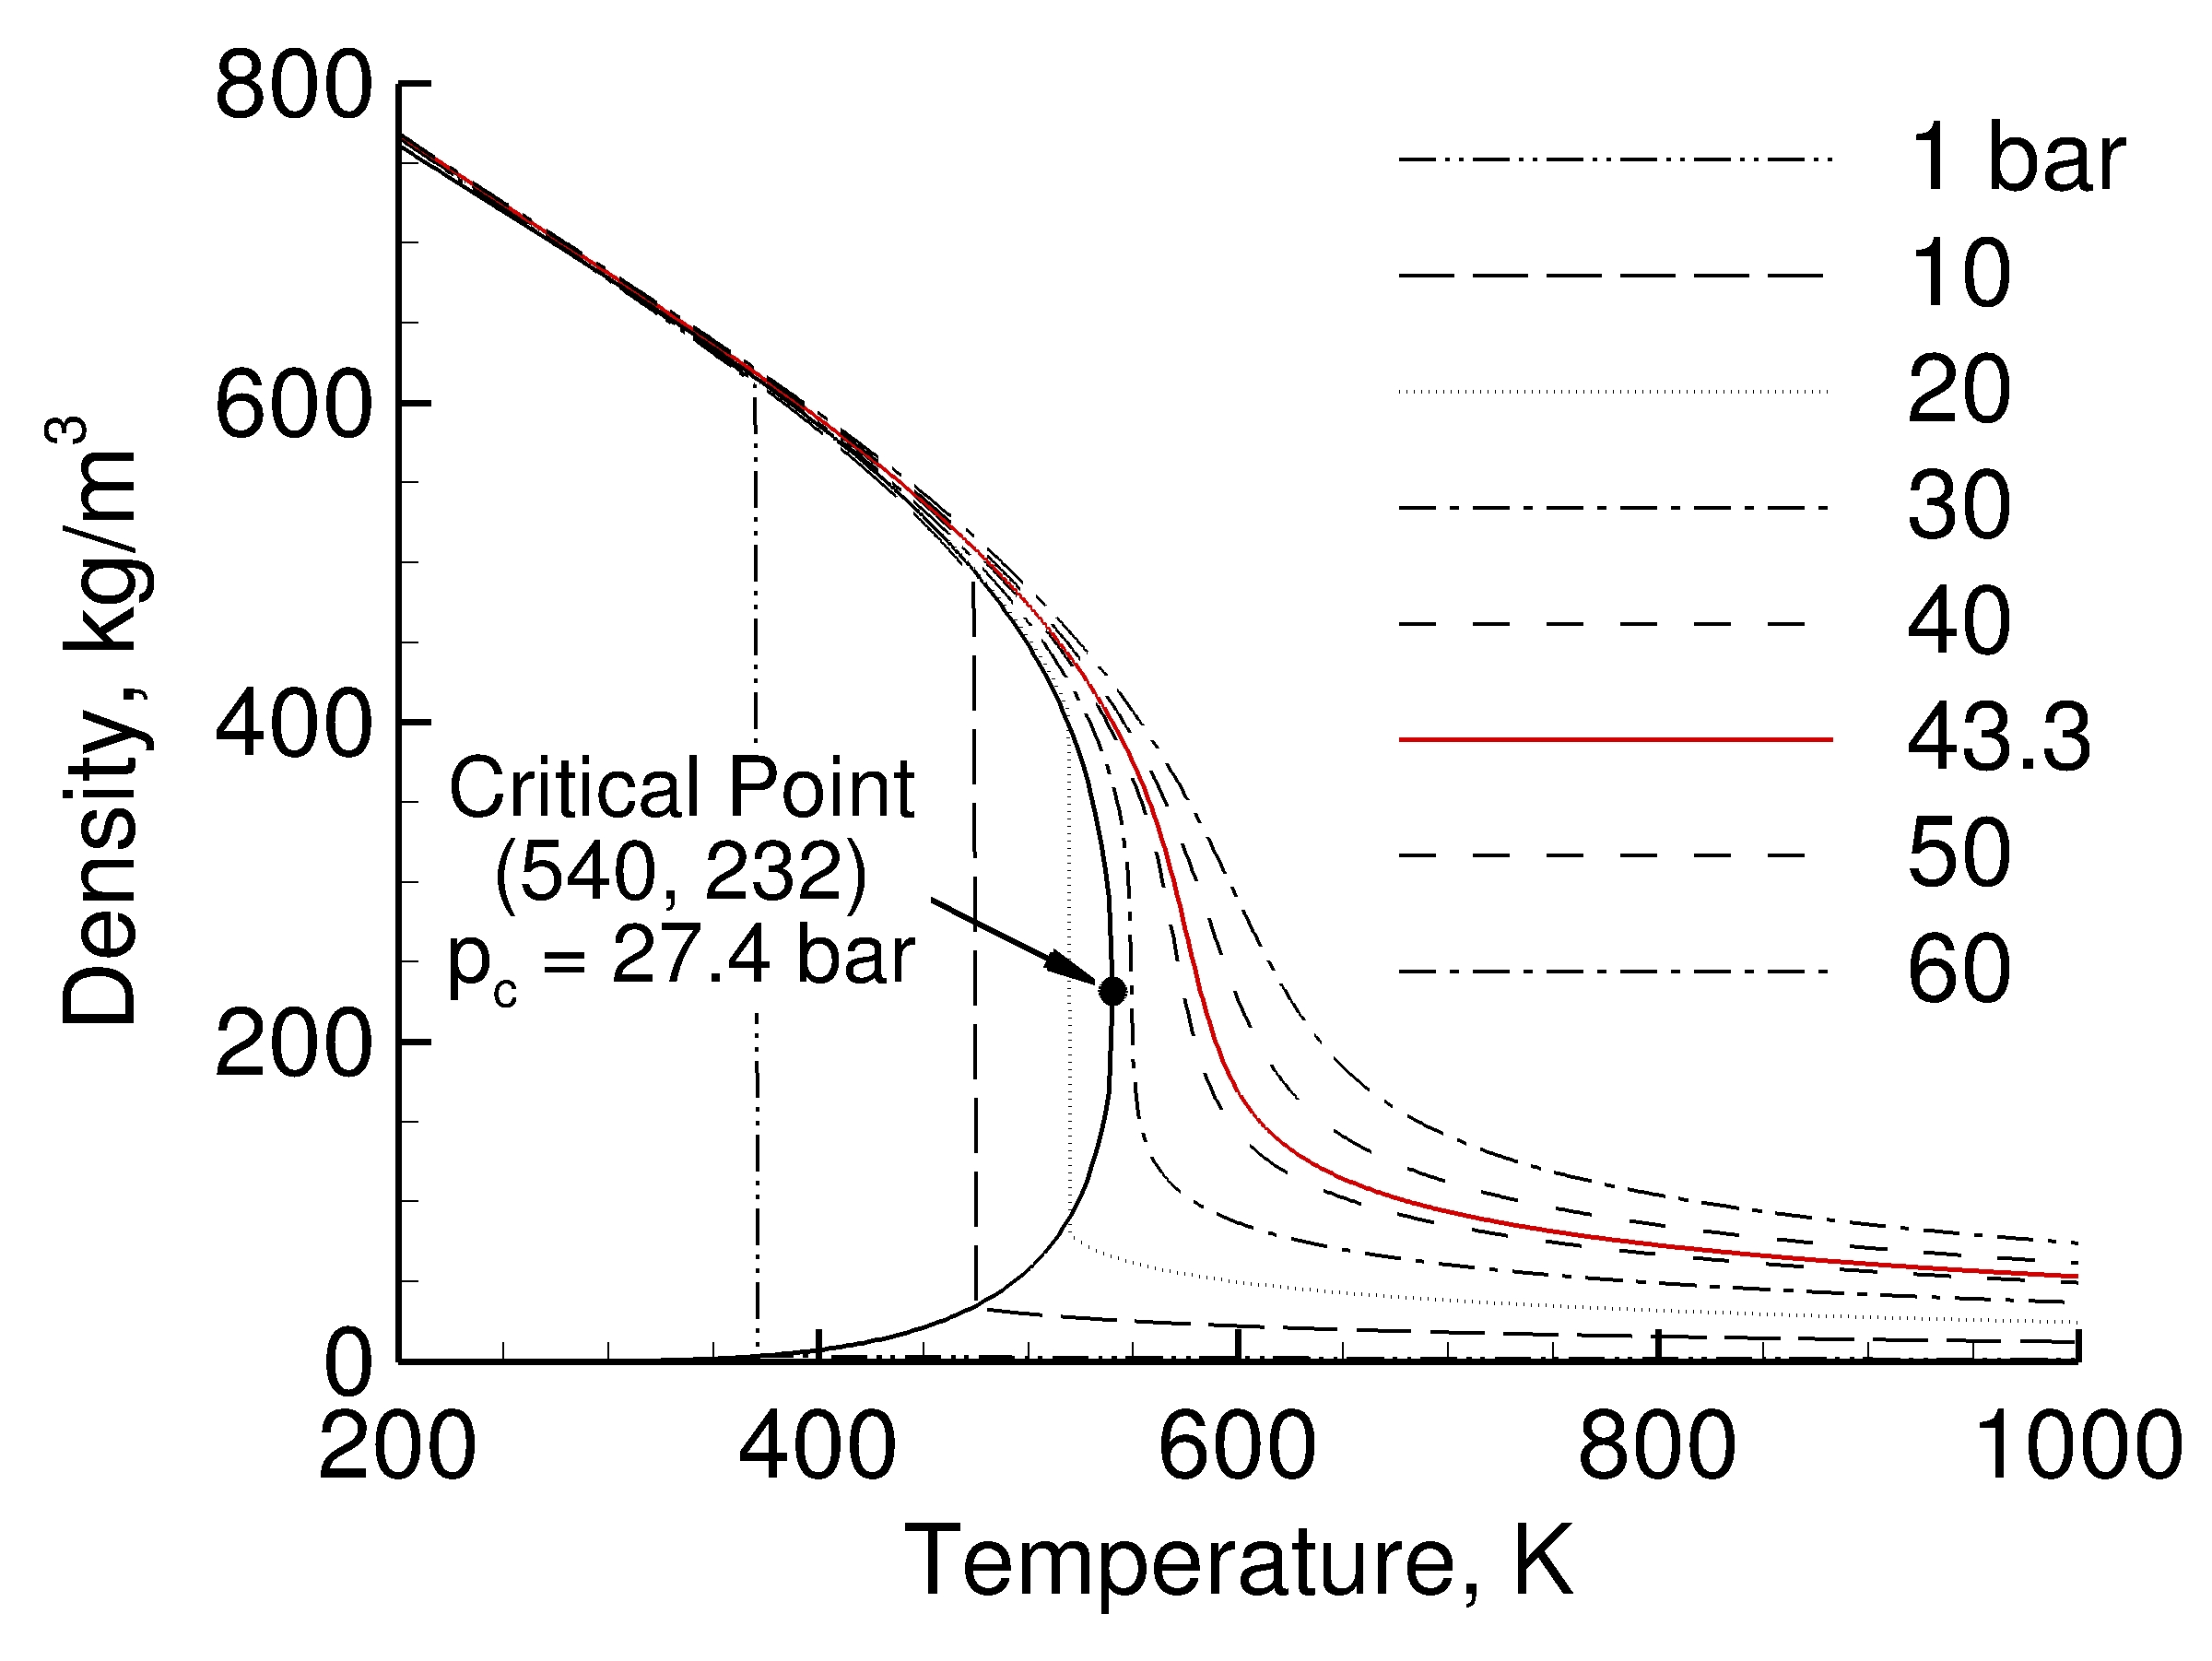
\includegraphics[width=192pt]{rho_T.jpg}
\caption{Density versus temperature of n-heptane.}
\label{rho_T}
\end{figure}

Single-column figures ({\em e.g.}, Fig.~\ref{rho_T}) should fit within the 2.67 in (67.7 mm) column width. Double-column figures ({\em e.g.}, Fig.~\ref{engine_fig}) should be sized for legibility, and the image must fit within the 5.67~in (144~mm) full text width. Figures are numbered sequentially using Arabic numerals. Figure captions use 8pt font with 10pt spacing.

Single- and double-column tables are inserted similarly. The font size throughout a table is 8pt, with 10pt line spacing. Table~\ref{engine} is an example of a single-column table, and Table~\ref{mechanisms} is an example of a double-column table.

\begin{table}[h!] \small
\caption{Engine specifications and operating conditions.}
\centerline{\begin{tabular}{lc}
\hline 
Description (units)                       & Value      \\
\hline
Bore (mm)                                  & 86          \\
Stroke (mm)                               & 86          \\
Connecting rod (mm)                   & 159        \\ 
Geometric compression ratio (-)    & 8.9         \\ 
Engine speed (r/min)                   & 1300       \\
Intake manifold pressure (kPa)     & 95          \\
Global equivalence ratio               & 0.2         \\
\hline 
\end{tabular}}
\label{engine}
\end{table}

Equations are numbered sequentially in the order in which they appear. Recent {\em Proceedings} papers can be consulted for appropriate equation formatting. Equation (1) is an example of a numbered equation. The Reynolds number, $Re$, is defined as:
\begin{equation}
Re \equiv UL/\nu ,
\end{equation}
where $U$ is a characteristic velocity, $L$ is a characteristic length, and $\nu$ is the fluid kinematic viscosity.

\section{Some example text} \addvspace{10pt}

The text in this section is taken from \cite{kazmouz21}. It is included here so that the text will carry over across two more pages. There are no formatting instructions in this section.

\begin{figure*}[h!]
\centering
\vspace{-0.4 in}
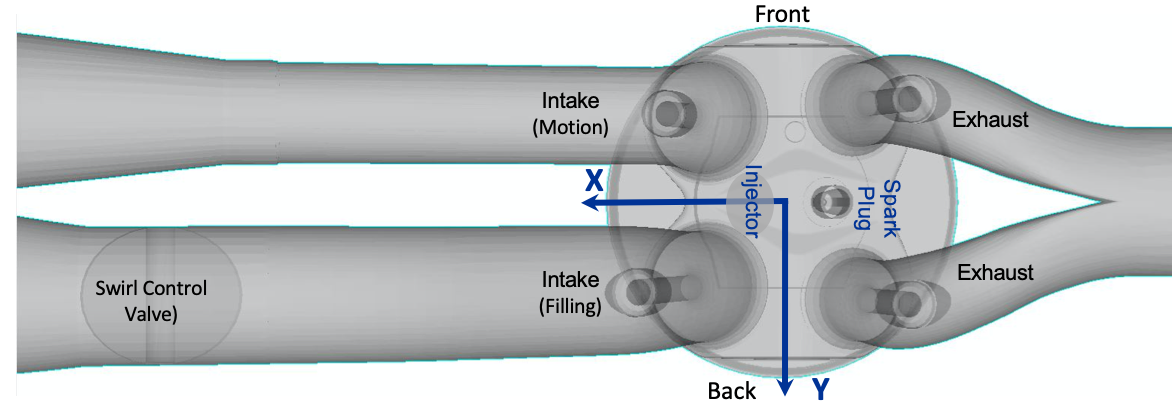
\includegraphics[width=300pt]{engine.png}
\vspace{10 pt}
\caption{Engine configuration (top view).}
\label{engine_fig}
\end{figure*}

Globally fuel-lean, stratified combustion in direct-injection spark-ignition (DISI) engines has the potential to reduce fuel consumption and carbon-dioxide emissions, compared to conventional stoichiometric homogeneous-charge engines. Issues include cycle-to-cycle variations (CCV) and criteria pollutant emissions, which require that the engine be calibrated to operate at conditions that are suboptimal for efficiency.

CCV have been studied extensively, using both experimental and computational approaches. In the case of homogeneous reactants, it has been shown that the early flame development largely determines the outcome of the combustion event. Most published CCV work has focused on the vicinity of spark plug at the time of ignition and the early flame development.

Spray-guided DISI (SG-DISI) engines operating in stratified mode offer additional complexities. The fuel is injected late, with appropriate timing and targeting to yield a flammable mixture at the spark plug at the time of ignition, and spark timing is limited to a narrow window after the end of injection. Exhaust-gas recirculation (EGR) may be used to control NOx, leading to even higher levels of CCV. It has been found that misfires in a SG-DISI engine correspond to cases where a flame kernel is initialized by the spark, but the kernel fails to fully develop into a propagating turbulent flame because it is advected away from the flammable mixture. Also, in the absence of in-cylinder fuel injection, in-cylinder turbulence levels increase in direct proportion to engine speed. In contrast, the turbulence level was found to increase by only 30\% with a doubling of engine speed in a late-injection SG-DISI engine. This implies that the heat release associated with the main combustion event in a stratified SG-DISI engine is determined by the mixing and turbulence induced by the injection event. In-cylinder swirl has been shown to reduce variability as the engine speed is increased in a SG-DISI engine. Swirl generates a repeatable vortex near the spray centerline, which redistributes momentum, and thus reduces variability, but increases soot formation. Swirl and tumble also can lead to asymmetrical fuel distributions.

The engine is a four-valve, four-stroke-cycle, single-cylinder, optically accessible spark-ignition engine with direct in-cylinder fuel injection (Fig.~\ref{engine_fig}). One intake port has a swirl-control valve that is used to modify the large-scale in-cylinder flow structure. Two of the eight spray plumes straddle the spark plug. The engine can be operated with early fuel injection, or in spray-guided stratified mode with late fuel injection.

Here a globally fuel-lean part-load stratified operating condition is considered, for which experimental results over 350 consecutive cycles are available. The fuel is an iso-octane/toluene blend; the toluene is included to enable equivalence-ratio measurements. Engine specifications and operating conditions are summarized in Table~\ref{engine}. 

\section{Acknowledgements, supplementary material, and references} \addvspace{10pt}

The Acknowledgements, Supplementary material (if included), and References section headings are not numbered. The font and spacing are the same as those for regular section headings.

For references, BibTeX can be used in the usual way. Here the references are provided in the file \verb+PCI_LaTeX.bib+. Several examples of references are included there. Recent {\em Proceedings} papers can be consulted for details concerning reference citing and formatting. The font size in the References section is 8pt with 10pt line spacing. The \verb+pci.bst+ bibliography style file should be used (included in this directory); this is identical to Elsevier's \verb+elsarticle-num.bst+. 

Note that titles are to be included for journal articles. Those were removed in error at the final stage of typesetting for Volume 38. The intent is that they will be retained in Volume 39. In the event that a paper is accepted for publication in the {\em Proceedings}, links will be added in the final published paper to directly access each of the references, where available.

\section{Nomenclature and appendix} \addvspace{10pt}

A nomenclature section and appendix are rarely included in {\em Proceedings} papers, because of length limitations. In the event that a nomenclature section is included, it should appear before the first numbered section heading under the unnumbered section heading “Nomenclature.” 
 
If an appendix in included, it should appear immediately before the references under the unnumbered section heading ``Appendix.''

The formatting for these section headings should be the same as that used for the Acknowledgements and Supplementary material.

\begin{table*}[ht] \small
\centering
\caption{\label{C2:MCP} Chemical mechanisms for multicomponent fuels.}
\begin{tabular}{cccccc}
\hline
\text{First author} & \text{Fuels or molecules}                                                      & \begin{tabular}[c]{@{}c@{}} \text{\# of species} \\ \text{/}\text{\# of reactions}\end{tabular}        & \text{\begin{tabular}[c]{@{}c@{}}Validation \\ cases\end{tabular}} & \text{Reference}     & \text{\begin{tabular}[c]{@{}c@{}}Mechanism \\ designation \end{tabular}}                       \\ \hline
O. Abianeh        & TRF-Ethanol                                                              & 62 / 194    & LFS                                                                       & \cite{abianeh2015development}   & A62               \\
H. Wang          & TRF-PAH                                                                  & 109 / 543       & LFS, HCCI,DICI                                                            & \cite{wang2015reduced}       & W109                  \\ 
J.C.G. Andrae           & TRF-Ethanol                                                         & 143 / 672       & LFS,HCCI                                                                  & \cite{andrae2009hcci}        & A143                \\ 
J.C.G. Andrae           & TRF-Ethanol                                                          & 1121/4961       & ST                                                                        & \cite{andrae2008development}  & A1121    \\ \hline
\end{tabular}
\label{mechanisms}
\end{table*}

\acknowledgement{Acknowledgments} \addvspace{10pt}

This LaTeX template was modified by Dan Haworth in September 2021, starting with a template that had been created by Joe Oefelein for earlier {\em Proceedings} volumes. Figure~\ref{rho_T} was also taken from that source. Figure~\ref{engine_fig} and Table~\ref{engine} were provided by Samuel Kazmouz from \cite{kazmouz21}, and Table~\ref{mechanisms} is based on a table provided by Jun Han.

Use the acknowledgement environment defined in the template for this section, not \verb+\section*+. 

\acknowledgement{Supplementary material} \addvspace{10pt}

If supplementary material is submitted along with the manuscript, that should be noted here. In the event that the manuscript is accepted for publication in the {\em Proceedings}, a DOI link to the online supplementary material will be included in the published paper.

Use the acknowledgement environment defined in the template for this section, not \verb+\section*+. 


% -------------------------------------------------------------------- %
% -------------------------------------------------------------------- %
% -------------------------------------------------------------------- %

 \footnotesize
 \baselineskip 9pt

% -------------------------------------------------------------------- %
% -------------------------------------------------------------------- %
% -------------------------------------------------------------------- %

\bibliographystyle{pci}
\bibliography{PCI_LaTeX}

% -------------------------------------------------------------------- %
% -------------------------------------------------------------------- %
% -------------------------------------------------------------------- %

\newpage

\small
\baselineskip 10pt

% -------------------------------------------------------------------- %
% -------------------------------------------------------------------- %
% -------------------------------------------------------------------- %

% -------------------------------------------------------------------- %
% -------------------------------------------------------------------- %
% -------------------------------------------------------------------- %

\end{document}

% -------------------------------------------------------------------- %
% -------------------------------------------------------------------- %
% -------------------------------------------------------------------- %
